\section{Audio and Heartbeat} 
\label{audio_and_heartbeat}
The audio and heartbeat system runs concurrently with the rest of the program. On an operating system supporting neither processes nor threads this means using interrupts to stop normal execution and perform tasks on the side.\\
\par
The idea is to configure the hardware to trigger a hardware interrupt at a regular interval. This interrupt is caught by a system called PIC which transforms it into a software interrupt. The software interrupt ID is used as an offset in a vector to look up a function belonging to the engine. At this point, the CPU is stopped (a.k.a: interrupted) from doing whatever it was doing (likely running the 3D renderer), and it starts running the interrupt handler which is called an ISR\footnote{Interrupt Service Routine}. We now have two systems running in parallel.\\
\par
\begin{figure}[H]
\centering
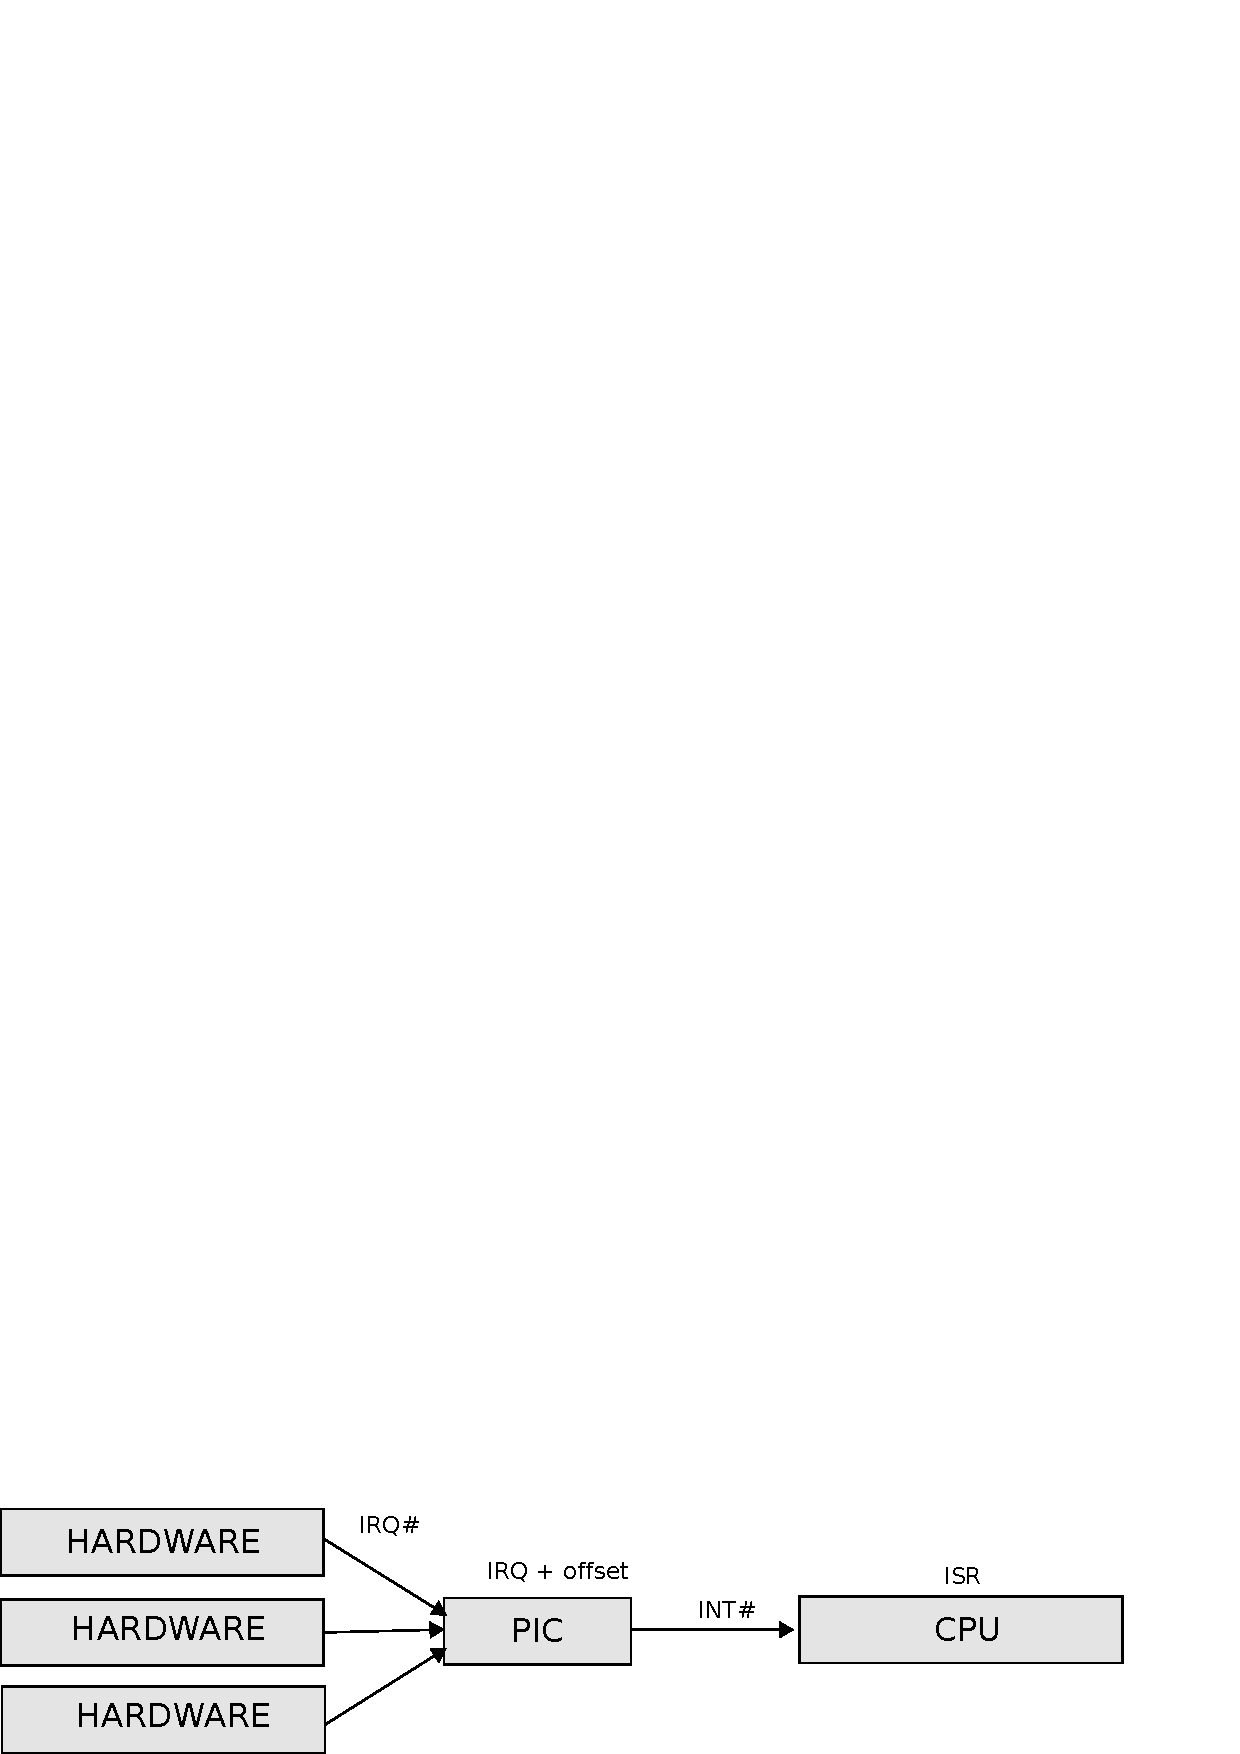
\includegraphics[width=\textwidth]{imgs/drawings/irqs/explanationsvg.pdf}
 \end{figure}
\par
\par
 Since interrupts keep triggering constantly from various sources, an ISR must make a choice with what should happen if an IRQ is raised while it is still running. There are two options.  The ISR can decide it needs a "long" time to run and disable other IRQs via the IMR \footnote{Interrupt Mask Register}. This path introduces the problem of discarding important information such as keyboard or mouse inputs. Alternately, the ISR can decide not to mask other IRQs and do what it is supposed to do as fast as possible, keeping in mind the routine can be stopped anywhere (and never resumed.)\\
 \par
 Wolfenstein 3D uses the latter approach and keeps tasks in its ISR very small and short. To this effect everything in the audio and heartbeat system is written in assembly and avoids "heavy" processing.

\subsection{IRQs and ISRs}
The IRQ and ISR system relies on two chips: the Intel 8254 which is a PIT \footnote{Programmable Interval Timer} and the Intel 8259 which is a PIC \footnote{Programmable Interrupt Counter}. The PIT features a crystal oscillating in square waves. On each period, it decrements its three counters. When a counter hits zero it generates an IRQ\footnote{Interrupt Request Line: Hardware lines over which devices can send interrupt signals to the CPU.}. One counter is connected to the buzzer and generates sounds, a second counter is connected to the RAM to automatically perform something called "memory refresh"\footnote{Without frequent refresh, DRAM will lose its content. This is one of the reasons it is slower and SRAM is preferred in caching system.}, and the third counter is connected to the PIC.\\
\par
\begin{figure}[H]
\centering
 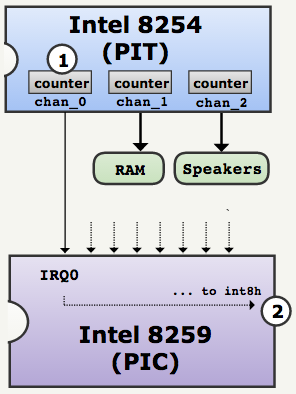
\includegraphics[width=.5\textwidth]{imgs/drawings/heatbeats.pdf}
 \end{figure}
\par

The PIC's hardware IRQ-0 to IRQ-8 are mapped to the Interrupt Vector starting at Offset 8 (resulting in mapping to software interrupts INT08 to INT0F.)\\

\par
\begin{figure}[H]
\centering
\begin{tabularx}{\textwidth}{ X X  }
  \toprule
  \textbf{INT} & \textbf{Type} \\ \bottomrule
0 & System timer \\
1 & Keyboard controller \\
3 & Serial port COM2 \\ 
4 & Serial port COM1 \\
5 & Line print terminal 2 \\
6 & Floppy controller \\
7 & Line print terminal 1 \\
8 & RTC timer \\
12 & Mouse controller \\
13 & Math co-processor \\
14 & ATA channel 1 \\
15 & ATA channel 2  \\
\bottomrule
\end{tabularx}

\end{figure}
Above are INTs and associated routines. Notice \#8 which is associated with the RTC Timer. This usually updates the operating system clock. Because IRQ\#8 was hijacked, operating system clock was wrong after running a game and remained so until the PC was rebooted.\\
\par
Using these two chips and placing its own function at Interrupt Vector Table \#8, the engine can stop its runtime at a regular interval, effectively implementing a subsystem running concurrently with everything else.\\
\par
The engine can decide at what frequency to be interrupted, depending on the type of sound/music it needs to play (digitized sounds are much more taxing than music.) As a result, three different ISRs can be found at IVT \#8: 
\begin{enumerate}
\item \cw{SDL\_t0ExtremeAsmService} when running at 7000Hz, to play digitized (PCM) sound.
\item \cw{SDL\_t0FastAsmService} when running at 700Hz, to play music and FM sound effects.
\item \cw{SDL\_t0SlowAsmService} when running at 140Hz, to play sound effects on the beeper via PWM.
\end{enumerate}
\par



\subsection{PIT and PIC}
The PIT chip runs at 1.193182 MHz. This seems like an odd choice from the hardware designers, but has a logical origin. In 1980 when the first IBM PC 5150 was designed, the common oscillator used in television circuitry was running at 14.31818 MHz. As it was mass produced, the TV oscillator was very cheap so utilizing it in the PC drove down cost. Engineers built the PC timer around it, dividing the frequency by 3 for the CPU (which is why the Intel ran at 4.7Mhz), and dividing by 4 to 3.57Mhz for the CGA video card. By logically ANDing these signals together, a frequency equivalent to the base frequency divided by 12 was created. This frequency is 1.1931816666 MHz. By 1991, oscillators were much cheaper and could have used any frequency but backward compatibility prevented this.\\
\par














\subsection{Heartbeats}
Each time the interrupt system triggers, it runs another small (yet paramount) system before taking care of audio requests. The sole goal of this heartbeat system is to maintain a 64 bit variable: \cw{TimeCount}.\\
\par
\begin{minipage}{\textwidth}
\lstinputlisting[language=C,morekeywords={longword}]{code/timecount.c}
\end{minipage}
\par
It is updated at a rate of 70 units per seconds (to match VGA update rate of 70Hz). These units are called "ticks". Depending on how fast the audio system runs (from 150Hz to 7000Hz), it adjusts how much it should increase \cw{TimeCount}.\\
\par
Every system in the engine uses this variable to pace itself. The renderer will not start rendering a frame until at least one tick has passed. The AI system expresses action duration in tick units. The input sampler checks for how long a key was pressed, and the list goes on... Everything interacting with human players uses \cw{TimeCount}.\\













\subsection{Audio System}
The audio system is complex because of the fragmentation of audio devices it can deal with. The early 90s was a time before Windows 95 harnessed all audio cards under the DirectSound common API. Each development studio had to write their own abstraction layer and id Software was no exception. At a high level, the Sound Manager offers a lean API divided in two categories: one for sounds and one for music.\\
\par
\begin{minipage}{\textwidth}
\lstinputlisting[language=C,morekeywords={longword}]{code/sound.h}
\end{minipage}
\par
But in the implementation lies a maze of functions directly accessing the I/O port of four sound outputs: Adlib, SoundBlaster, Buzzer, and Disney Sound Source. All belong to one of the three supported families of sound generators: FM Synthesizer (Frequency Modulation), PCM (Pulse Code Modulation) or PWM (Pulse Width Modulation.)\\


\subsection{Music}
Playing music is not too messy since only PCs equipped with a Yamaha YM3812 FM synthesizer can play tracks (a.k.a: with an Adlib or a SoundBlaster inside.) As SoundBlaster made its programming interface compatible with Adlib there is only one code path to both cards. There is not a lot of magic here since this uses a piece of well-designed hardware dedicated to this specific task. There are a few cool tricks, though.\\
\par
The music system streams data to the sound cards. Music in the 90s was not in digitalized formats like CD or MP3 nowadays (that would have taken too much storage space and bandwidth.) Instead music was stored as series of notes played on channels simulating instruments. The format used is close to the notorious MIDI but with a few variations and is called IMF\footnote{Id Music Format}. It is proprietary to id Software and designed with OPL2 in mind (the raw format is exactly what is sent to the Adlib/Soundblaster synthesizer with no transformations.) IMF has a hardcoded playback rate and music notes are played at 700 Hz.\\
\par
Hardware limitations dictated certain aspects of music design. The FM synthesizer (OPL2) has 9 channels (a.k.a instruments) yet the composer, Bobby Prince, was asked to use only channels 1 to 8. This little trick allows for multiplexing music and sound effects on AdLib cards since it leaves channel 0 available at all times (the SoundBlaster plays sound differently.)\\




\subsubsection{OPL2/YM3812 Programming}
\ref{IMF_explanation}
\par
Programming the OPL2 output is esoteric to say the least. AdLib and Creative did publish SDKs but they were expensive.  Documentation was sparse and often cryptic. Today, they are almost impossible to find.\\
\par
The OPL2 is made of 9 channels capable of emulating instruments. Each channel is made of two oscillators: a Modulator whose outputs are fed into a Carrier's input. Each channel has individual settings including frequency and envelope (composed of attack rate, decay rate, sustain level, release rate, and vibrato.) Each oscillator can also pick a waveform (these characteristic forms are what gave the YM3812 its recognizable sound.)\\
\par
 To control all of these channels, a developer must configure the OPL2's 244 internal registers. These are all accessed via two external I/O ports. One port is for selecting the card's internal register and the other is to read/write data to it.\\
\par
\begin{minipage}{\textwidth}
\lstinputlisting[language=C,morekeywords={longword}]{code/audio_ports.c}
\end{minipage}
\par
When the AdLib was released in 1986, developers were instructed to send data "as fast as possible". At 4.77Mhz, a PC was unable to out-pace the Adlib. Yet as CPUs got faster, issues started to arise and the card was unable to keep up. The Programming Guide was amended.\\
\par

\begin{fancyquotes}
After writing to the register port, you must wait twelve cycles before sending the data; after writing the data, eighty-four cycles must elapse before any other sound card operation may be performed\protect\footnotemark.
 \bigskip \\
 Alternatively you can issue one IN instruction.
 \bigskip \\
 \end{fancyquotes}
\\
\footnotetext{http://www.oldskool.org/guides/oldonnew/sound .}
\par
Later, reliable specs were published.\\
\par
\begin{fancyquotes}
Wait three point three (3.3) microseconds for the address, and twenty-three (23) microseconds for the data.\\
 \end{fancyquotes}
 

\par
The engine does not know about any of the details of the OPL2. There is zero abstraction layer or transformation here. An IMF song is made of a series of messages containing exactly the values to write to the register and data ports of the OPL2. Each message is four bytes:\\
\par
\begin{minipage}{\textwidth}
\lstinputlisting[language=C,morekeywords={longword}]{code/adlib_message.c}
\end{minipage}
\par
The \cw{reg} byte is sent to port \cw{0x388}, the \cw{data} byte is sent to \cw{0x389}, and the \cw{delay} 2 bytes are used to tell how much time to wait before sending the next register/data to the card. The stream is hard-coded at 700Hz and the delay is expressed in this unit: a value of 700 means to wait 1000ms before sending another command. Whenever there is music playing the engine runs at no less than 700Hz (it can run at 7000Hz if it is also playing digitized sound but that results in no-ops for music playback.) A value of zero means the next message should be sent immediately.\\
\par
Overall, music is simple to execute because almost everything has been pre-processed via IMF. Every time the audio system wakes up, it checks if music packets should be sent, sends them, and moves on to the sound effects.










\section{Sound Effects}
Sound effects are where things become complicated. None of the cards use the same format and audio configurations are numerous. The sound settings screen illustrates how complex this is.
\par
\begin{figure}[H]
\centering
 \fullimage{audio/audio_settings.png}
 \end{figure}
\par
Sounds are stored in three formats. Once for PC Speaker, once for AdLib, and once for SoundBlaster/Disney Sound Source in the \cw{AudioT} archive created by Muse. Sounds are segregated by format but always stored in the same order. This way a sound can be accessed in three formats by using \cw{STARTPCSOUNDS} + \cw{sound\_ID} or \cw{STARTADLIBSOUNDS} + \cw{sound\_ID}.\\

\par
\begin{minipage}{\textwidth}
\lstinputlisting[language=C,morekeywords={longword}]{code/muse_header.c}
\end{minipage}
\par
Strangely, only PC speaker and AdLib sounds are stored in the \cw{AUDIOT.*} files, the digitized sounds are in the \cw{VMSWAP.*} archive. As a result, offset \cw{STARTDIGISOUNDS} is never used. Despite questioning the authors, it seems nobody can remember why.\\

\par



\subsection{Sound effects: AdLib}
AdLib only has a FM synthesizer, with sounds played on its Channel 0. Sounds are played the same way as music (via IMF) as previously described.












\subsection{Disney Sound Source system: PCM}
The Disney Sound Source is simple to program\footnote{The Programmer's Guide to the Disney Sound Source is a whopping 2 pages!} because it can do only one thing. It plays PCM audio in format 8 bits at 7000Hz on a single channel. That's it -- nothing more, nothing less. As soon as it is plugged in the parallel port, its 8 bit DAC will read from an internal 16 bytes deep FIFO and turn them into sound via its integrated loud speaker.\\ 
\par
Every time the audio system wakes, it reads the DAC status to check if the FIFO is full. If it is not, the engine pushes as many bits as possible until the FIFO is full and returns. When the FIFO empties, the Disney Sound Source stops making noise.\\
\par










\par
\subsection{SoundBlaster system: PCM}
Since the SoundBlaster also supports 7000Hz PCM, it uses the same sound effects files as the Disney Sound Source. However, it also features a DSP which is DMA capable. As a result, the CPU does not have to waste cycles transferring data. The audio system only has to ensure it is running at 7000Hz and pointing the DMA to the right memory address each time it crosses the end of a 16K segment via a DMA routine callback.
\par








\par
\subsection{SoundBlaster Pro system: Stereo PCM}
\par

On a "high-end" SoundBlaster Pro, the Mixer described on page \pageref{sbmixerpage} is used to simulate 3D sounds. The source of the sound is first rotated with the same formula seen on page \pageref{rotatematrix}. The player's position is used to generate two attenuation values (between 0 and 15) which are then packed in a byte and sent to the mixer. The difference of volumes tricks the player into perceiving the sound origin anywhere within the 180 degrees facing her.\\
\par 
\begin{minipage}{\textwidth}
\lstinputlisting[language=C]{code/setposition.c}
\end{minipage}
\par
\bu{Trivia :} Plugging in a SoundBlaster card was not enough to produce sound. This was before "plug \& play" was introduced by Windows 95. The user had to write a special line in the startup command of the PC (\cw{autoexec.bat}).\\
\par 
\begin{minipage}{\textwidth}
\lstinputlisting[language=C]{code/soundblasterconf.c}
\end{minipage}
\par
This line defines a variable \cw{BLASTER} which the engine retrieves and parses at runtime with \cw{getenv}. \cw{A} tells what port the card is using. \cw{I} gives away the interrupt vector it is associated with. Finally \cw{D} gives the DMA channel to use for data transfer. For all this to work the sound card had to be configured accordingly via its jumper connectors.
See \cw{SDL\_SBPlaySeg} and the ISR \cw{SDL\_SBService} 




 
\subsection{PC Speaker: PWM}
The hardware chapter described a problem for sound effects: the default PC speaker could only generate square waves, resulting in long beeps which are not acceptable for gaming.\\

\par
 \begin{fancyquotes}
  The PC speaker is normally meant to reproduce a square wave via only 2 levels of output (the speaker is driven by only two voltage levels, typically 0 V and 5 V). However, by carefully timing a short pulse (i.e. going from one output level to the other and then back to the first), and by relying on the speaker's physical filtering properties (limited frequency response, self-inductance, etc.), the end result corresponds to intermediate sound levels. This effectively allows the speaker to function as a crude 6 bit DAC, thereby enabling approximate playback of PCM audio.\\
  \par
  This technique is called pulse-width modulation (PWM).
 \end{fancyquotes}
\par
  
The idea is to approximate a signal using square waves. It is simpler to understand when the signal is a simple sinusoid:
\par
\begin{figure}[H]
\centering
 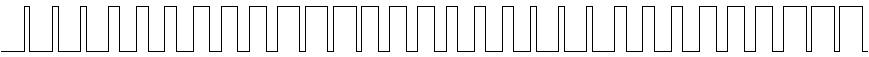
\includegraphics[width=\textwidth]{imgs/drawings/pwm/sinuois.png}
 \caption{The original sound.}
 \end{figure}
\par

\par
\begin{figure}[H]
\centering
 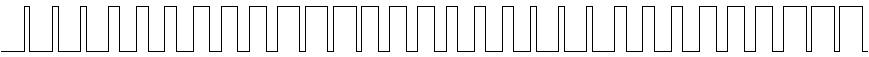
\includegraphics[width=\textwidth]{imgs/drawings/pwm/pwm_approximation.png}
 \caption{The same sound approximated with PWM.}
 \end{figure}
\par

To do this, the audio system once again relies on the PIT chipset. Counter 0 is used to trigger the audio system. Counter 1 is used to refresh the RAM periodically. Counter 2, however, is directly connected to the PC Speaker. The trick is to set this Counter 2 to square wave mode (Mode 3) so it will repeat after it triggers and program the desired square wave frequency. \\
\par
\begin{figure}[H]
\centering
\begin{tabularx}{\textwidth}{ X X  }
  \toprule
  \textbf{Mode} & \textbf{Type} \\ \bottomrule
1 & Hardware Re-triggerable One-shot\\
2 & Rate Generator\\
3 & Square Wave Generator\\
4 & Software Triggered Strobe\\
5 & Hardware Triggered Strobe\\
\bottomrule
\end{tabularx}
\caption{Available modes of a PIT counter.}
\end{figure}
\par 
When instructed to play a PWM sound effect, the audio system sets itself to run at 140Hz via PIC Counter 0. Every times it wakes up, it reads the frequency to maintain for the next 1/140th of a second and writes it to Counter 2. The frequencies to use are encoded as a stream of byte, the value of which is decoded as follows:\\
\par 
\begin{minipage}{\textwidth}
\lstinputlisting[language=C]{code/pwm.c}
\end{minipage}
\par
In the assembly, three I/O ports are accessed:\\
\par
\begin{minipage}{\textwidth}
\lstinputlisting[language=C]{code/pwm_code_header.c}
\end{minipage}
\par
Notice how the $ * 60$ is not calculated. Once again the engine tries to save as much CPU time as possible by using a bit of RAM. The frequency is read from a lookup table \cw{pcSoundLookup}:\\
\par
\begin{minipage}{\textwidth}
\lstinputlisting[language=C]{code/pcSoundLookup.c}
\end{minipage}
\par
Notice how \cw{6b} (\cw{10110110}) is sent to the PIC Command register (\cw{pcTAccess}=\cw{0x43}):
\begin{itemize}
	\item \cw{10} = Target Counter 2.
 	\item \cw{11} = High \& low byte of counter updated.
	\item \cw{011} = Square Wave Generator.
	\item \cw{0} = 16 bit mode.
\end{itemize}
\par
\begin{minipage}{\textwidth}
\lstinputlisting[language={[x86masm]Assembler}]{code/pwm_code.asm}
\end{minipage}
\par
While the end result was not great, it was better than a beep\footnote{LucasArts obtained surprisingly good results for their game Monkey Island. See the video "LGR - Evolution of PC Audio - As Told by Secret of Monkey Island", https://www.youtube.com/watch?v=a324ykKV-7Y.}.\\
\par

\bu{Hidden feature :} The source code features an audio code path which plays PCM digitized sound via the PC Speaker.\\

\par 
\begin{minipage}{\textwidth}
\lstinputlisting[language=C]{code/sound_fork.c}
\end{minipage}
\par
Notice the \cw{SDL\_PCPlaySample} path allowing PCM to be played on the buzzer. This codepath shipped but was never enabled\footnote{You can still hear it thanks to youtube: "Wolfenstein 3D Hack - Digitized PC Speaker Sound Effects" at https://www.youtube.com/watch?v=1BtlsjJRnFU .}. We may speculate it was a matter of overhead but the cost would have been the same as the Disney Sound Source playback. Questioning the authors of the game did not shed light on this mystery.\\
\par















